\subsection{MicroNet Tools}
\label{sub:tools}

The MicroNet tools are a collection of Eclipse plug-ins. Eclipse was chosen due
to the primary Java nature of MicroNet. This allows to develop Java \mss{} very
quickly. But the MicroNet Tools also offer a solution to integrate other
technologies into a \ms{} application. This language independence is
accomplished by using Json as a low level information exchange format. As long a
a technology supports Json it can participate in the application. Another
requirement is that the technology has access to the message broker.

Since the user interface (UI) of an Eclipse plug-in is written using the Swing
Window Toolkit (SWT) library it can easily be exported to be a standalone tool
decoupled from Eclipse. With this approach it is possible to port the MicroNet
Tools to other Platforms as long as they support a JVM.

The MicroNet Tools have been completely developed within this last semester
thesis and are the major contribution to four of the hypotheses listed in
\autoref{sub:hypothesis}: The composition, deployment, simple development, and 
reproducibility hypotheses.

\subsubsection{Files and Folders Structure}

To allow loose coupling of a \ms{} application the MicroNet makes a few
assumptions on how to organize files and folders:

\begin{itemize}
  \item The eclipse workspace folder must contain one project folder for each
  \ms{}
  \item For automated integration of a \ms{} its project folder must be either a
  Java/Maven project or must contain a Dockerfile.
 \item One shared folder to exchange the Shared Model and the Service API must
 be present
\end{itemize}  

\begin{figure}
	\centering
	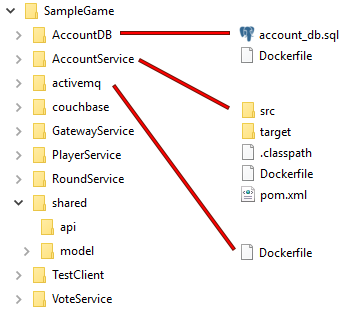
\includegraphics[width=9cm]{images/tools/folder_structure}
	\caption{Example folder structure of a MicroNet application workspace.}
	\label{fig:folder_structure}
\end{figure}

\autoref{fig:folder_structure} shows an example folder structure of a MicroNet
application workspace. The shared folder in this case is simply a folder within the
workspace. The figure also shows three canonical examples of project folders.
The AccountDB folder represents a containerized PostgreSQL database. The
AccountService folder is a standard MicroNet Maven/Java service project. The
activemq folder contains only a Dockerfile which is the minimal requirement to
participate in a MicroNet application.

\subsubsection{Annotations}

MicroNet annotations allow to define a service in a very lean way. A service is
defined by annotating a arbirtary class with the
@MessageService(uri=``mn://service\_name'') annotation. Within the service class
methods can be annotated @MessageListener(uri=``/api\_method'') to act as
message handlers. \todo{Screenshot}

MicroNet annotation are basically an implementation of the design by contract
pattern. A service defines preconditions on request payloads and
defines postconditions on response payloads.
 
 \paragraph{Annotation Processing}
 
Java Annotations can be either be used during run-time or processed during
compilation-time. MicroNet only processes annotations at compile-time. Since
Java version 6 the annotation processing process is tightly integrated into the
standard Java build process. This makes the annotation process platform
independent and can be reproduced in a standard java build, a Maven build or an
Eclipse build\footnote{Annotation processing is done by the Java compiler and
tests showed that the execution is slightly different for the mentioned build
systems.}.

Annotation processing is also the entry point for code generation. Even if no
annotation are present the code generation for the model can be done either way.

\subsubsection{Code Generation}

Code generation allows the developer to omit  the boiler plate code that is
needed to set up the service in the framework. This covers the setup of the
appropriate networking solution according to the environment and the generation
of the executable class of the \ms{}. This simplification allows the developer
to focus more on the actual domain logic of the \ms{}. It also spares the
developer in having to register the service within the application. The
registration is done implicit by the annotation processor.

Code generation is implemented using the Java Poet library. It allows for
typesafe generation of Java classes and is very easy to use. 

\paragraph{Service Generation}

The annotations that define message service and the message listeners are used
to build the executable class of a \ms{}. The executable class registers all
message listeners with the networking system. In addition the annotated @Start
and @Stop methods are called at application start respectively at service
termination. The generated main method encompasses the start/stop functionality
and the listener registration in a defined set-up sequence.

\paragraph{Model Generation}

The model generation process is completely independent from the service
generation and is used to translate the game model which is defined in Json to
java POJOs (plain old Java objects). This process can also be reproduced in
other programming languages by using similar mechanisms. 

The challenge is not the generation itself but the editing of the model that is
generated and its representation. \todo{correct references.}

\subsubsection{Code Assist}

The Code Assist plug-in helps the developer to keep track of functionality
provided by other services. It allows to enforce type-safety by using the pre-
and postconditions defined by the MicroNet annotations.

Code Assist is implemented by using the correspondent Eclipse extension point.
It allows to add custom entries to the code completion list box. This
functionality is used to offer the MicroNet API to the developer any time he
types ``mn://''. The proposals are filtered according to what the developer
types.

The type safety concept yet not implemented can be used in addition to verify is
the message exchange is adequate according to the pre- and postconditions of the
API. Upon violation the compiler can generate an error which forces the
developer to fix the issue before a build can be executed. Although possible the
implementation involves parsing the Java abstract syntax tree (AST) and this
effort is out of the scope of this thesis.\todo{screenshot}

\subsubsection{Service Explorer}

The service explorer helps the developer to get an overview over the whole
game application. It helps the manage the versions of services of the game
services as well as dependency management. The service explorer supports Java,
Maven and Docker projects.

The service explorer can also be used to quickly edit the configuration of
services. This includes the port configuration as well as service linkage for
the Docker overlay network.

The service explorer can also be used to compose the game application. This is
done by selecting if a service is part of the Maven build and/or part of the
Docker container build process.

\subsubsection{Launch Utility}

The launch utility brings order to the vast different possibilities of how to
orchestrate \ms{} application with containers. Many different configurations are
needed to develop, test and deploy a \ms{} application.

\paragraph{Local Native}

The native configuration runs or debugs a game application as a set of native
Java applications. This makes debugging very fast and the integration in Eclipse
provides many useful debugging tools. To launch multiple Java applications at
once the CDT Lanuch Group plug-in is used. It composes multiple launch
configurations into a single configuration. Upon start all contained
applications are started individually. No build step is needed for this
configuration.

In the native configuration it is easiest to run dependencies as standalone
installations on the host. Since the native configuration is solely used during
development this allows to also test the dependencies isolated from the composed
application.

\paragraph{Local Containerized}

The local containerized configuration is meant to reproduce the deployment
process on the local developer machine. For this purpose Maven and Docker
compose/swarm are used. 

A local Maven build of the complete application is done by aggregating the
individual Maven service projects into a master .pom file. The master .pom can
be used to build the whole application at once. Which services are aggregated to
the master .pom file can be configured via. the service explorer.

A local Docker is defined by a docker-compose file. The file is also defined by
configuring services via the service explorer. The build process is simply
invoked by building the docker-compose file.

To run the local containerized application the local docker engine can be used.
Docker-compose is installed native with most docker installation or can be
installed separately. If the application is started using Docker compose or
docker swarm makes a minor difference but several differences in networking or
container linkage require to test bock approaches for an application.

\paragraph{Cloud Containerized}

The final step of \ms{} application deployment is cloud deployment. The idea
behind containerized application is that this process is meant to be fully
equivalent on different systems. This also holds for \ms{} driven \og{} and
therefore if the application is working with the local containerized
configuration the cloud configuration is only a few steps away.

Due to the restriction mentioned in \todo{ref budget} the production environment
of \mn{} is a virtual server in the HSR network. The deployment process is
mainly based on this environment. Since this a very general setup the process
can easily be reproduced on other environments.

In order to deploy a MicroNet \ms{} application the developer must perform these
steps under the assumption that the server runs a fresh Linux installation.

\begin{itemize}
  \item Install: Docker Engine, Java, Maven and Git
  \item Initialize docker swarm (master and worker machines)
  \item Pull the game application repository (containing all service projects
  and the shared folder)
  \item Build the application using the master .pom file (annotation processing
  is performed during this step)
  \item Containerize the application using docker-compose API
  \item Launch the application in the docker swarm using the docker stack API 
\end{itemize}

This sounds like a lot of steps but in fact most of these steps only take a few
seconds and only consist of very few console commands.

\subsubsection{Model Editor}

The model editor is the last feature that was introduced in MicroNet tools. It
is the final solution on how to cope with logical \ms{} composition in a visual
way. Since the game model is of very theoretical nature it is not suited to be
edited directly in its underlying Json format. Because of this the model editor
is especially important to allow convenient editing of the game model underlying
a game application.

The model edit is basically a graph editor visualizing a direct representation
of the game graph to allow to extending and changing the graph. The graph has
three root nodes for which each span a model tree.

\paragraph{Parameter Code List}

The parameter code tree is simply a flat list of String constants which defines
all parameter codes used throughout the application. This global approach allows
to substitute the parameter codes strings with numbers which is more space
efficient. Since parameters are used very often this has a noticeable impact on
bandwidth requirements.

The datatype of the parameters is defined by using templates of the shared
model.

\paragraph{Template Tree}

The template tree allows to edit the game type graph. Object Types defined using
the template tree can be used for message transfer and persistence. Templates
are descriptions of domain objects that can be used to generate data classes
using code generation.

A template consists of a set of fields of the following types: STRING, NUMBER,
BOOLEAN, CHAR, ENUM, LIST, SET, MAP, and COMPONENT. The types are derived from
the Java types since they are well documented and can be redefined in other
programming languages using the Java language specification.

The COMPONENT type can be any other template type. In this case the component is
contained in the data class as a struct and not as a reference. Also template
types can be derived from other templates. This is realized using Java
inheritance.

\paragraph{Prefab Tree}

The prefab tree is the ``physical'' representation of the game graph. It
contains actual instances of template types. This can be used by game designer
to pre-define game objects. The prefab tree is directly compatible with the
serailization component provided by MicroNet. This allows services to use the
generated model to directly serialize and de-serialize game objects from the
database or from payloads and parameters during message transfers.

The prefab tree can either be persisted in the file-system or persisted in the
database. Either way the prefab approach allows for very convenient and
consistent handling of game data.

